\subsection{24 августа. А/л <<Узункол>>}
\textit{Метеоусловия: утром пасмурно, днём дождь, вечером переменная облачность.}


\begin{figure}[h!]
	\centering
	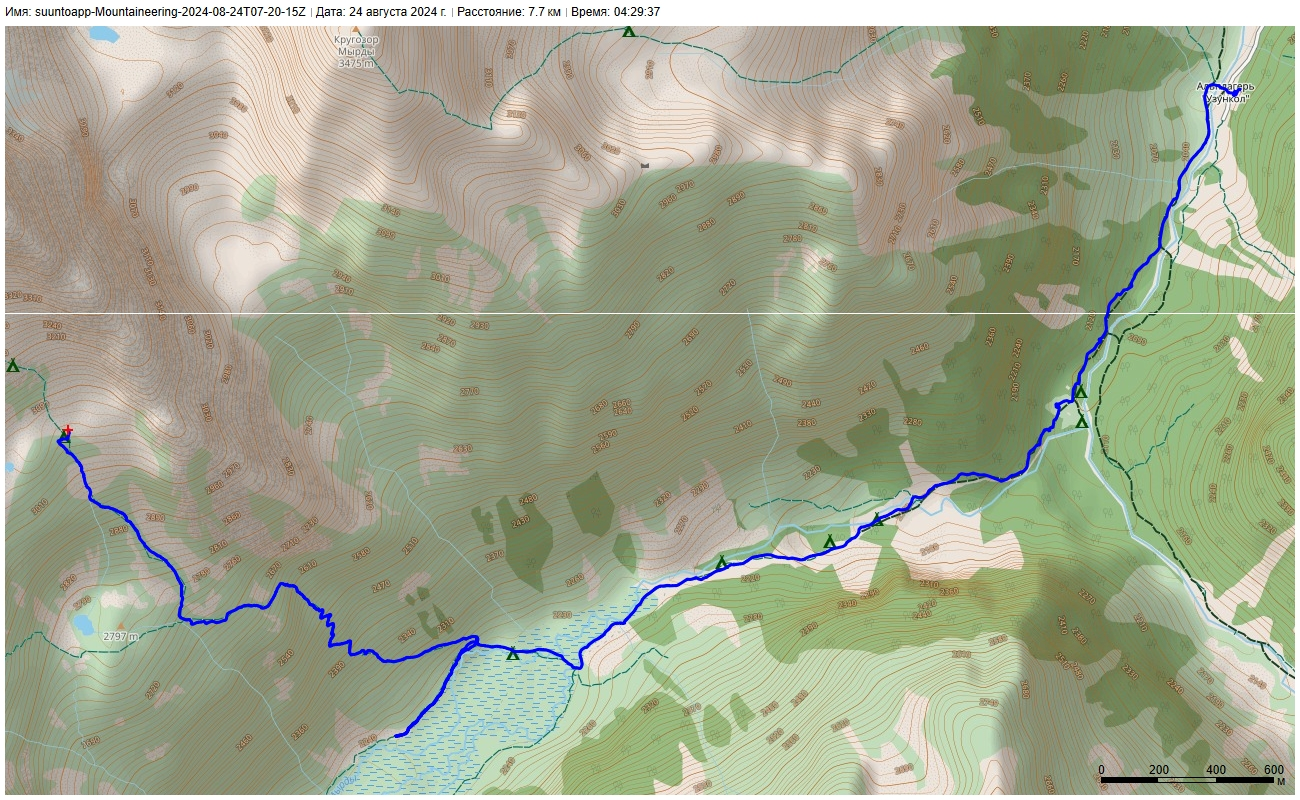
\includegraphics[angle=0, width=0.7\linewidth]{../pics/mini_maps/24}
	\label{fig:mini_24}
\end{figure}



Подъём в 08:00, выход в 10:20. Сегодняшняя наша цель~--- спуститься в а/л <<Узункол>> и устроить там полуднёвку.

Спускаемся по хорошо  набитой тропе, спуск трудностей (помимо зарослей малины и чабреца) не вызывает.

\begin{figure}[h!]
	\centering
	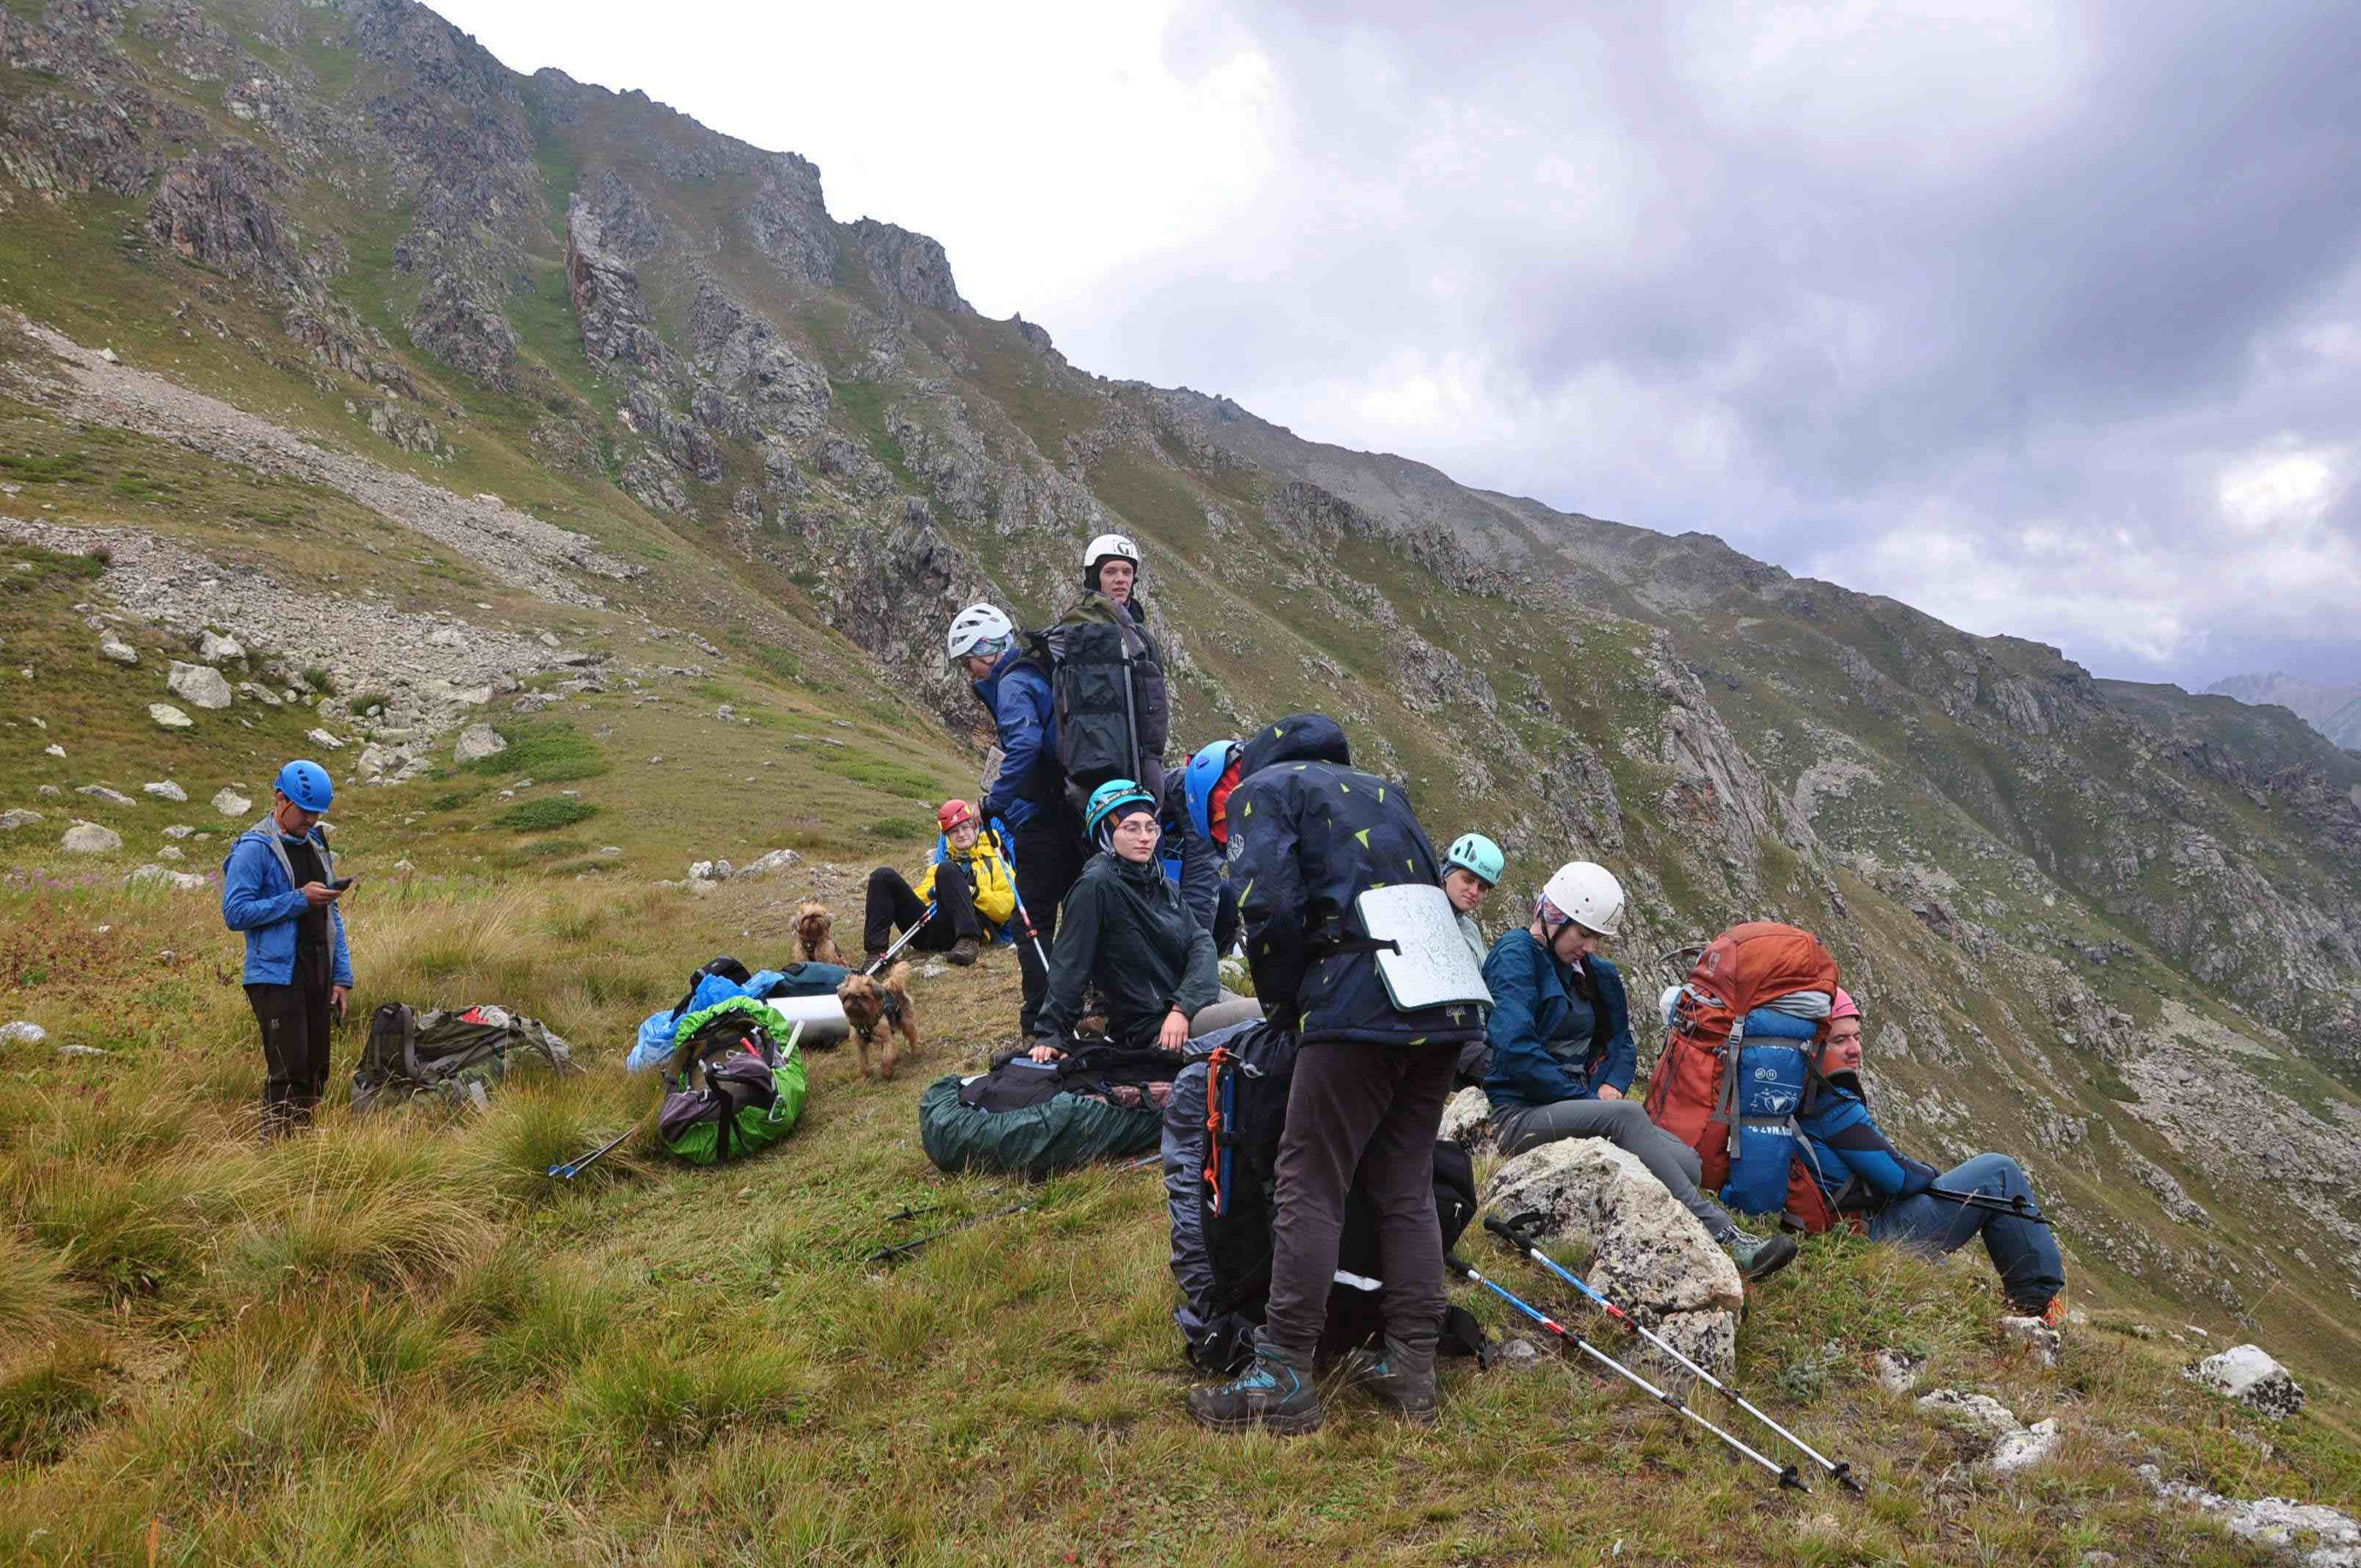
\includegraphics[width=0.7\linewidth]{../pics/DSC_0104.jpg}
	\caption{Группа на спуске в д.р. Мырды}
	\label{fig:DSC_0104.jpg}
\end{figure}

\begin{figure}[h!]
	\centering
	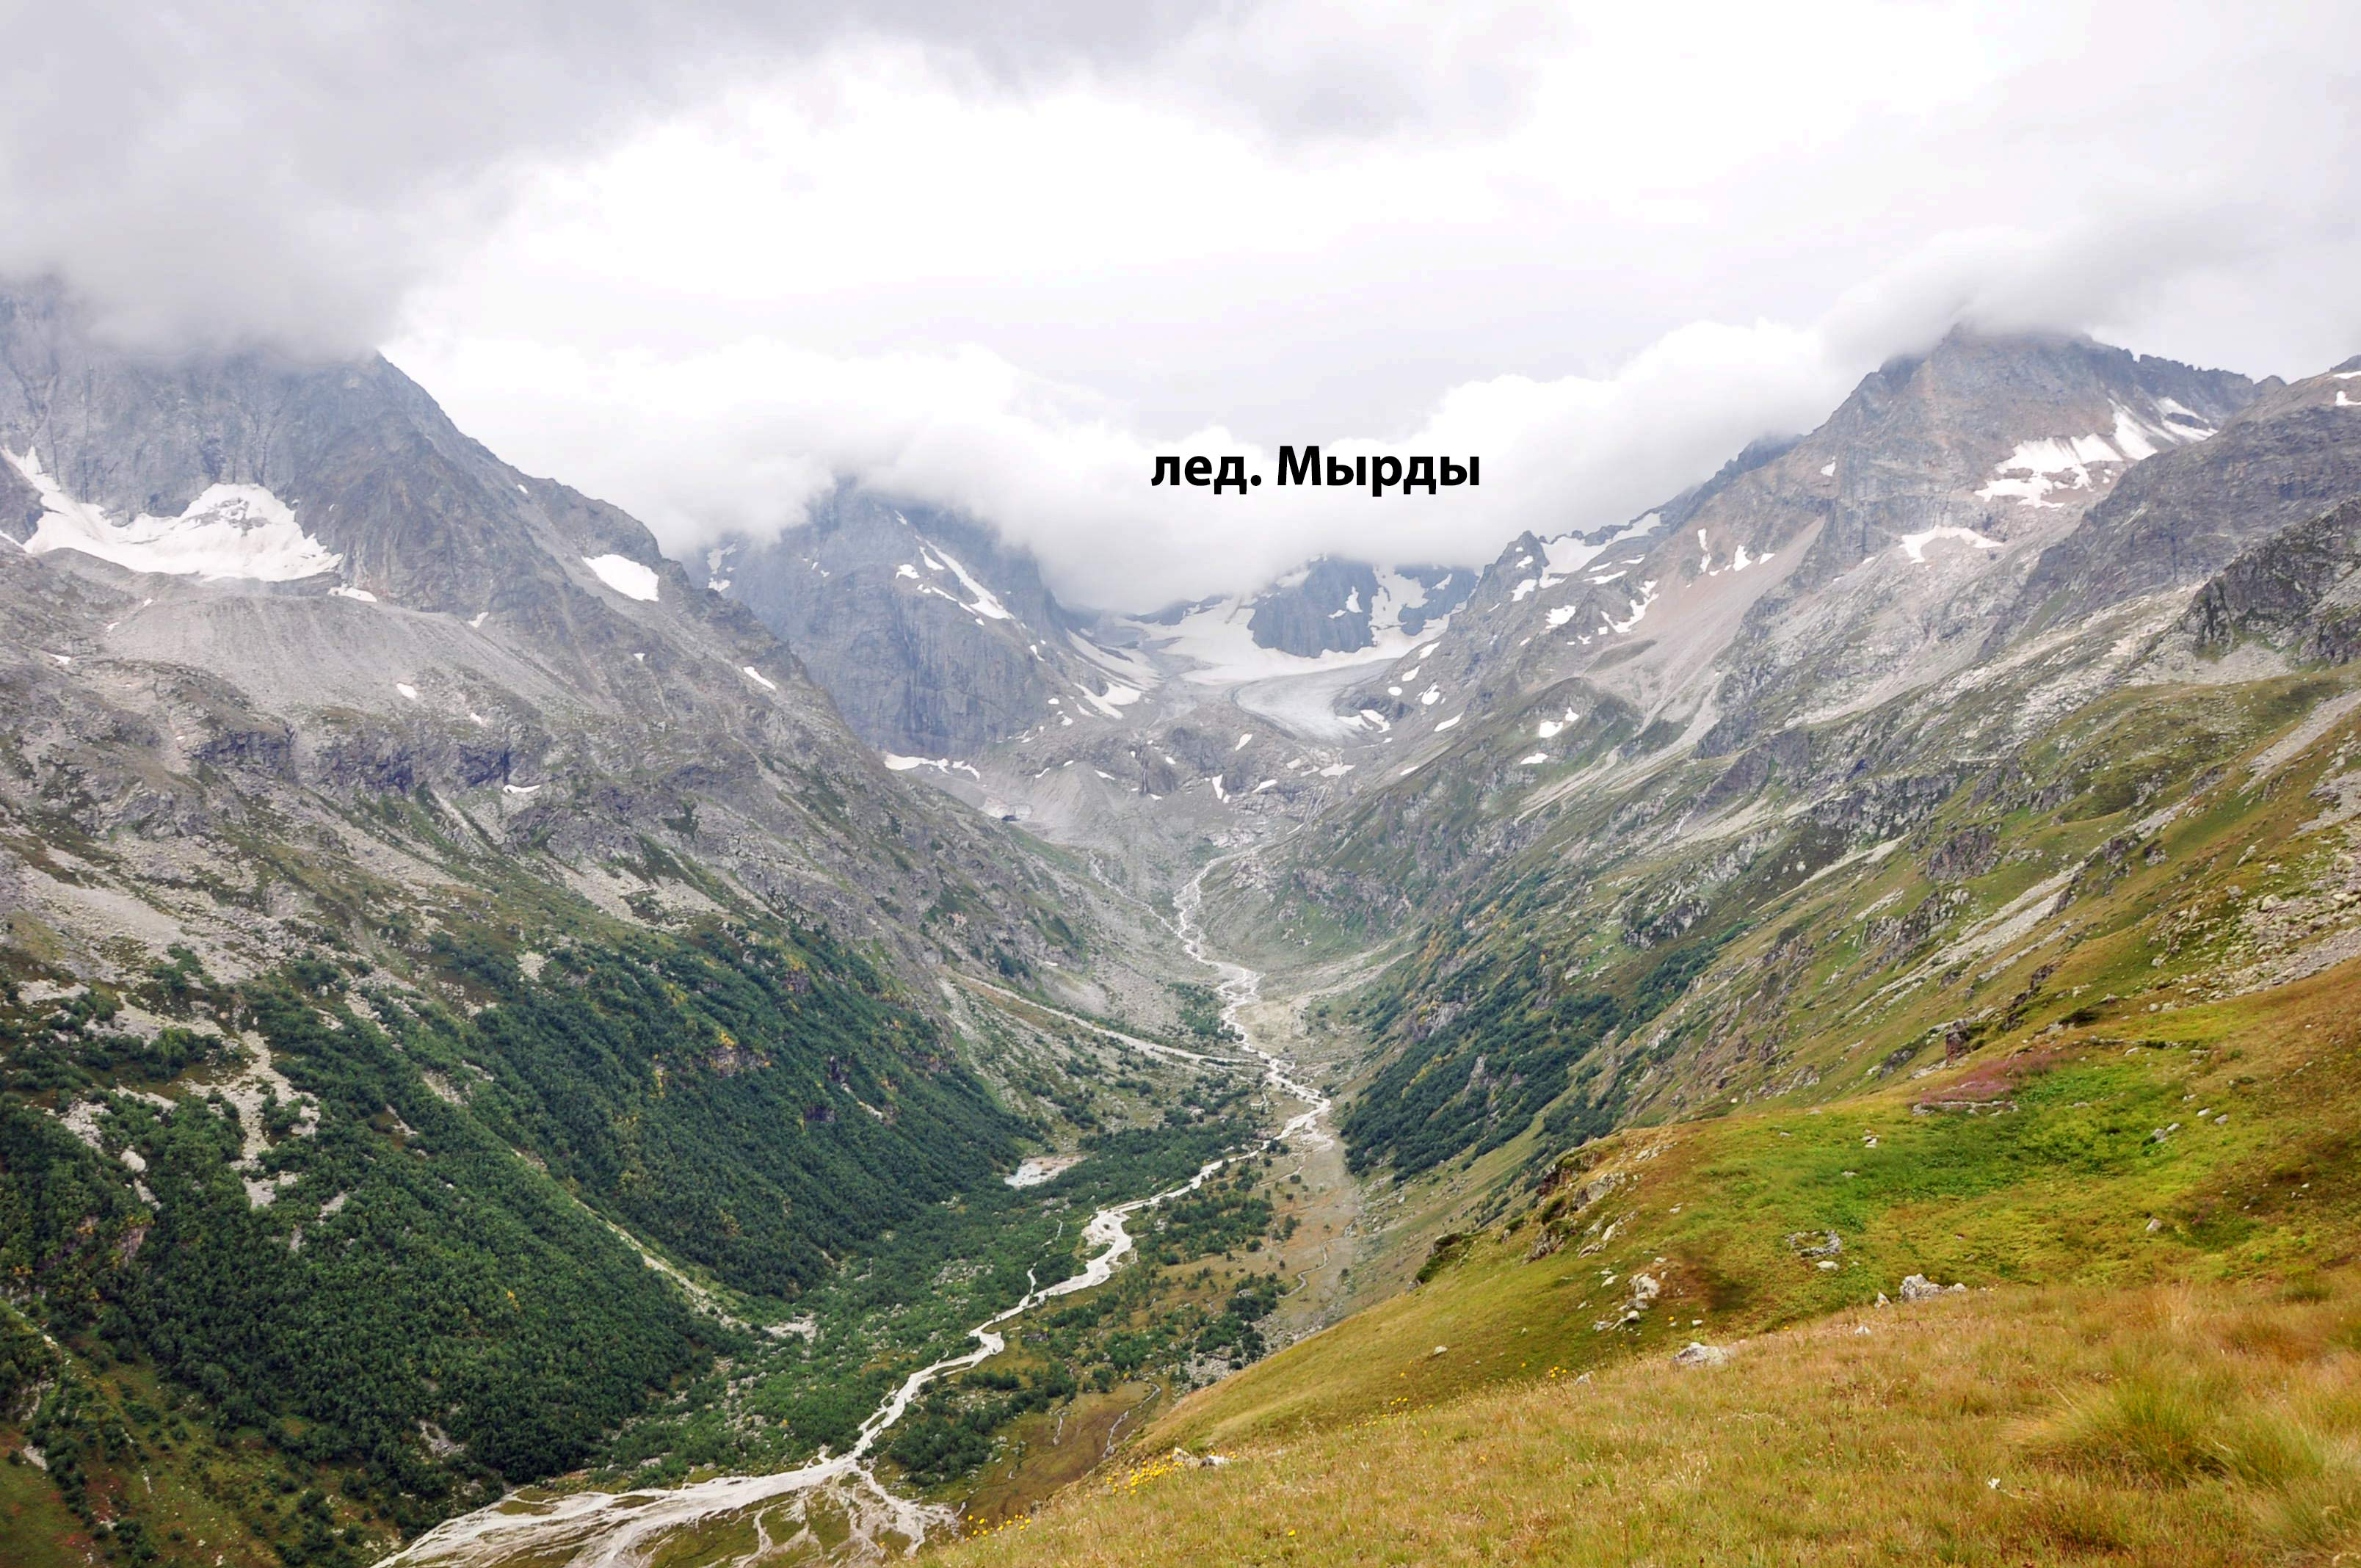
\includegraphics[width=0.7\linewidth]{../pics/DSC_0107.jpg}
	\caption{Верховья р. Мырды}
	\label{fig:DSC_0107.jpg}
\end{figure}

Спустились на дно долины в 12:50. Попутно нас обгоняли многочисленные группы гуляющих налегке туристов из а/л <<Узункол>>.

Спустившись к реке, устроили привал, в ходе которого часть группы прошла 400 м вверх по течению в поисках <<нарзанных источников>> N~43.264012\degree, E~42.137496\degree~(рис. \ref{fig:DSC_0111.JPG}). Фактически, мы нашли несколько источников воды, богатой железом и с сильным запахом сероводорода: по вкусовым ощущениям эта вода не шла ни в какое сравнение с нарзанными источниками в д.р. Махар около т/б <<Глобус>>.

\begin{figure}[h!]
	\centering
	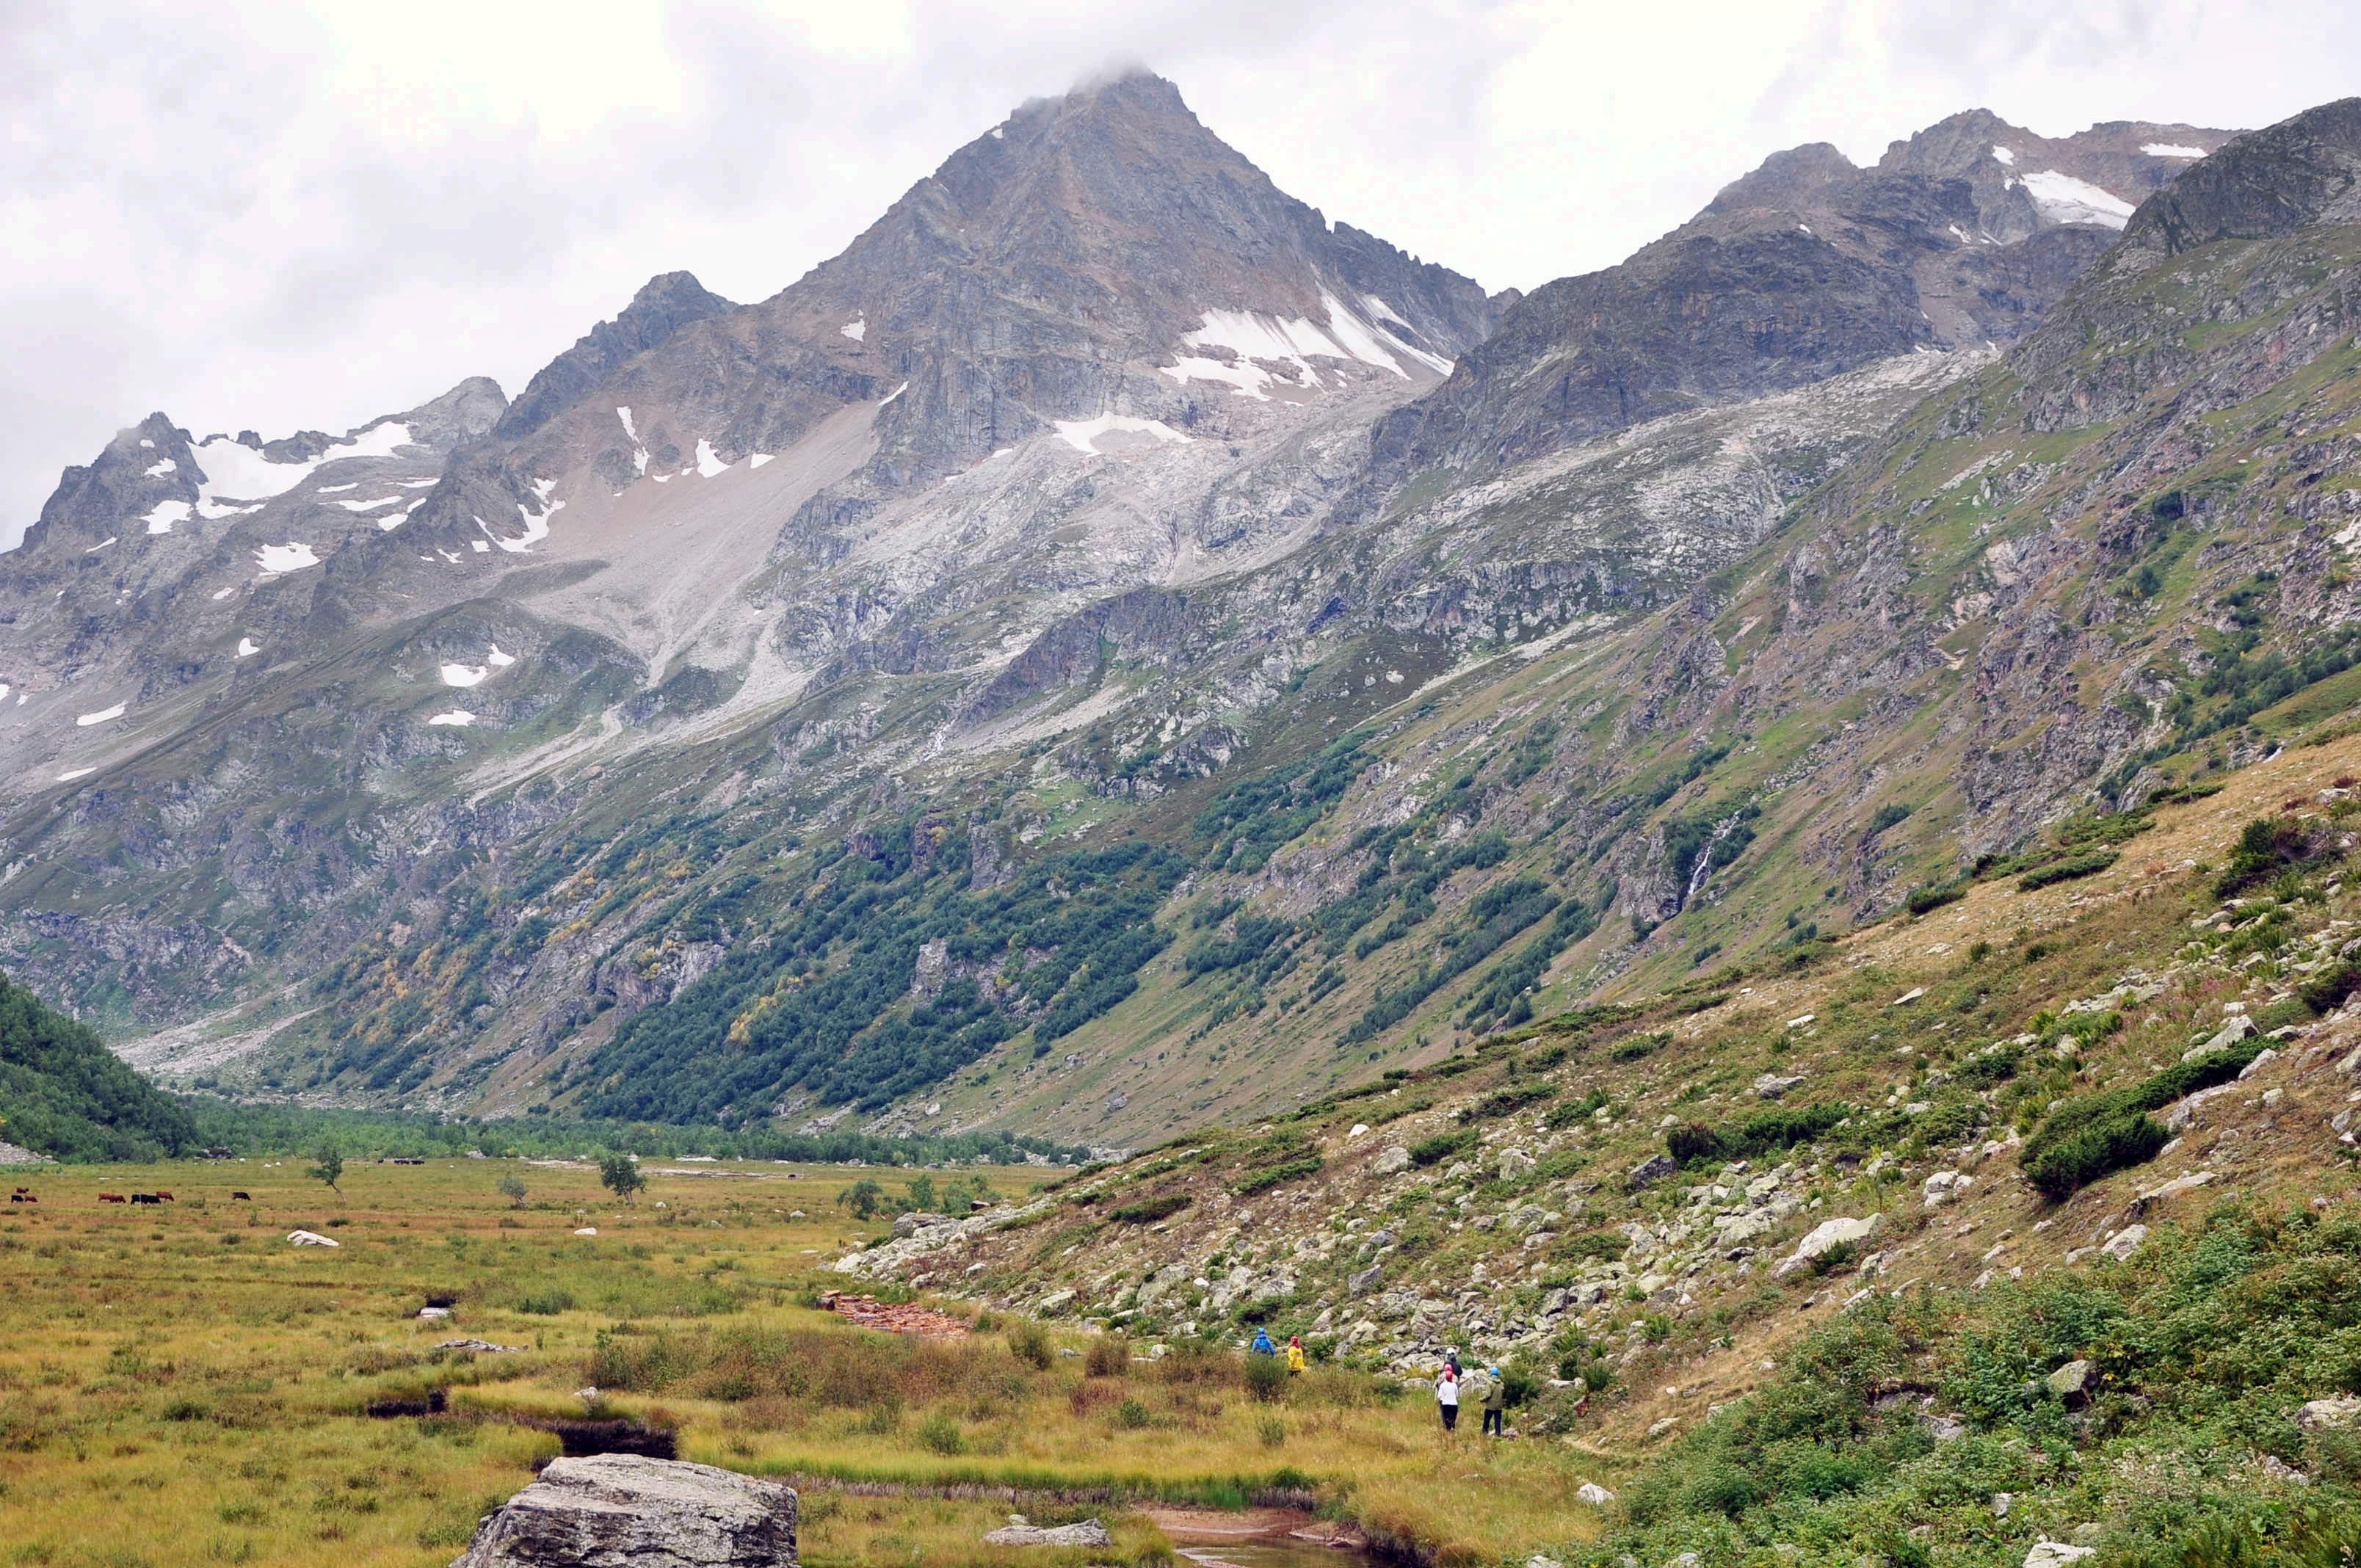
\includegraphics[width=0.7\linewidth]{../pics/DSC_0111.JPG}
	\caption{Группа в поисках нарзанных источников}
	\label{fig:DSC_0111.JPG}
\end{figure}

Далее переходим р. Мырды по хорошему пешеходному мосту на правый берег и идём по автомобильной дороге. Разрушенный мост через р. Мырды, ведущий на левый берег и упоминавшийся в отчёте \cite{Korolyov2018} как разрушенный, в настоящий момент восстановлен, его координаты N~43.271433\degree, E~42.159714\degree. Рядом находится автомобильный брод.

В 14:20 подходим к погранзаставе. Проверка документов занимает менее 10 минут, после чего идём к альплагерю, где оказываемся в 14:45.

Народу в альплагере много, но места под палатки есть. С нас берут 500~\faRub~с человека за ночь. В стоимость, помимо места под палатку, входит горячий душ, возможность подзарядить гаджеты и воспользоваться интернетом (последнее~--- с 19:00 по 23:00). За хранение заброски с нас взяли 100~\faRub~за мешок в день. Вечером мы воспользовались баней (2500~\faRub~с группы за час). Остаток дня потратили на отдых, стирку, распределение заброски и празднование годовщины свадьбы руководителя и зам. руководителя.



\clearpage